\documentclass{beamer}

\mode<presentation>
{
  \usetheme{CambridgeUS}
  \usecolortheme{rose}

  \setbeamercovered{transparent}
}

\usepackage[english]{babel}
\usepackage[latin1]{inputenc}
\usepackage{times}
\usepackage[T1]{fontenc}
\usepackage{amsmath}
\usepackage{amsfonts}
\usepackage{caption}
\usepackage{natbib}
\usepackage{kbordermatrix}
\kbalignrighttrue

\beamertemplatenavigationsymbolsempty

\title[GCN]{}


% \subtitle
% {Presentation Subtitle} % (optional)
\author[Laplace]
       {%
         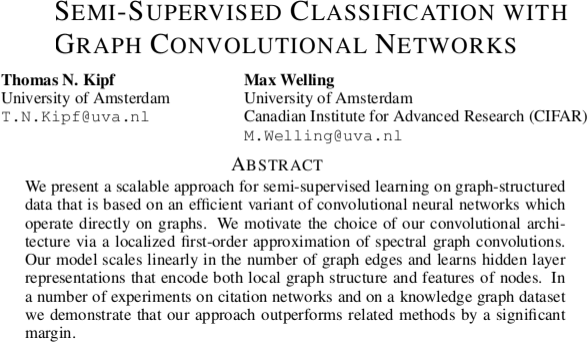
\includegraphics[width=1.0\textwidth, height=0.6\textheight, keepaspectratio]{img/article_header}~\\
         Pierre-Simon Laplace
       }
%% \institute[UNL] % (optional, but mostly needed)
%% {
%%   University of Nebraska-Lincoln
%% }
% - Use the \inst command only if there are several affiliations.
% - Keep it simple, no one is interested in your street address.

\date[\today] % (optional)
{\today}

\subject{Talks}
\pgfdeclareimage[height=0.5cm]{university-logo}{img/logo}
\logo{\pgfuseimage{university-logo}}


\AtBeginSubsection[]
{
  \begin{frame}<beamer>{Outline}
    \tableofcontents[currentsection,currentsubsection]
  \end{frame}
}

\begin{document}
\begin{frame}
  \vspace{-2.7cm}
  \titlepage
\end{frame}

\section{Introduction}
\begin{frame}{Why Do We Need Graph Convolutional Networks}
  \begin{figure}[ht]
    \centering
    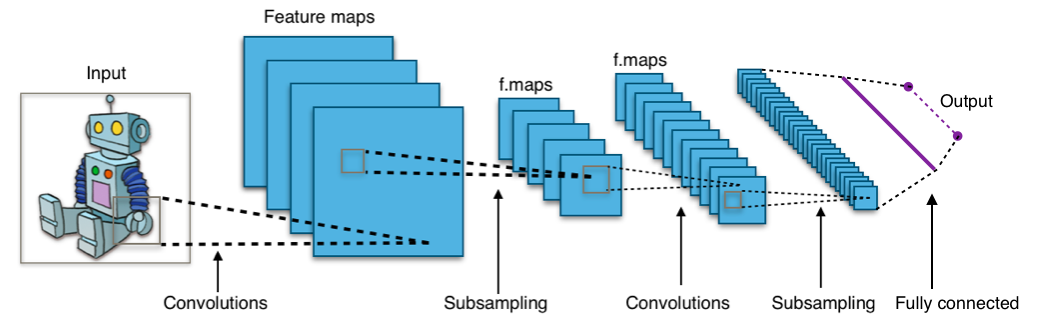
\includegraphics[width=1.0\textwidth,height=0.5\textheight, keepaspectratio]{img/cnn}
    \label{fig:cnn}
  \end{figure}
  \vspace{-1cm}
  \begin{minipage}[t]{.2\textwidth}
    \begin{figure}[ht]
      \centering
      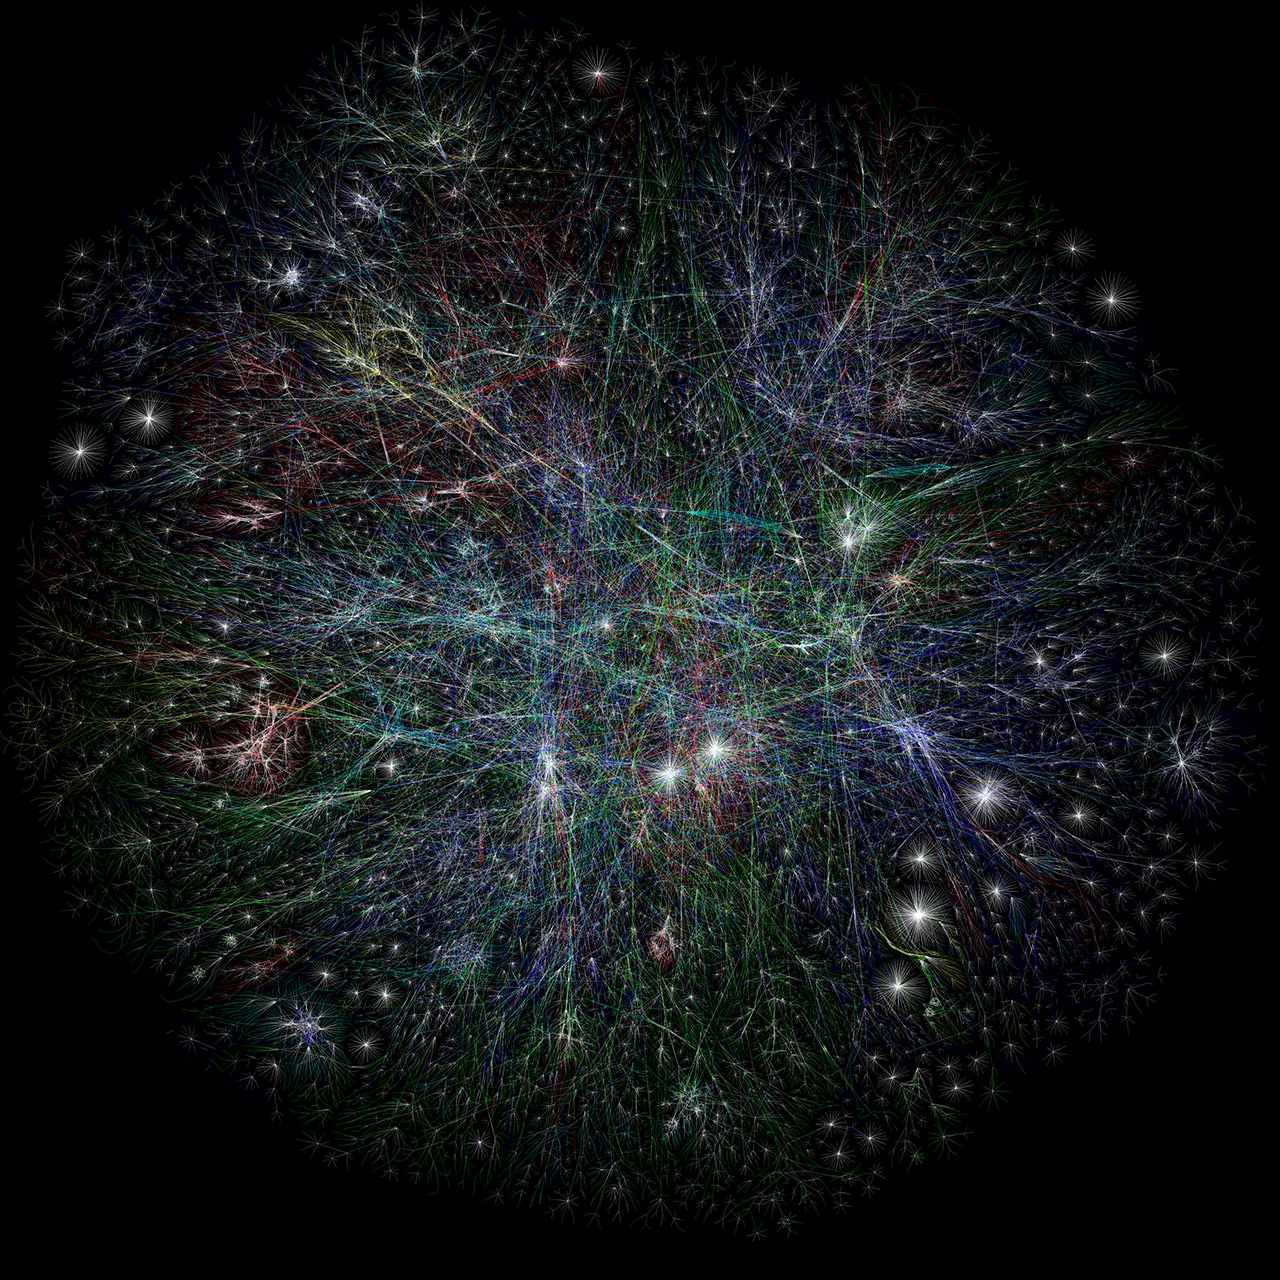
\includegraphics[width=1.0\textwidth]{img/internet_map}
      \label{fig:internet}
    \end{figure}
  \end{minipage}
  \begin{minipage}[t]{.3\textwidth}
    \begin{figure}[ht]
      \centering
      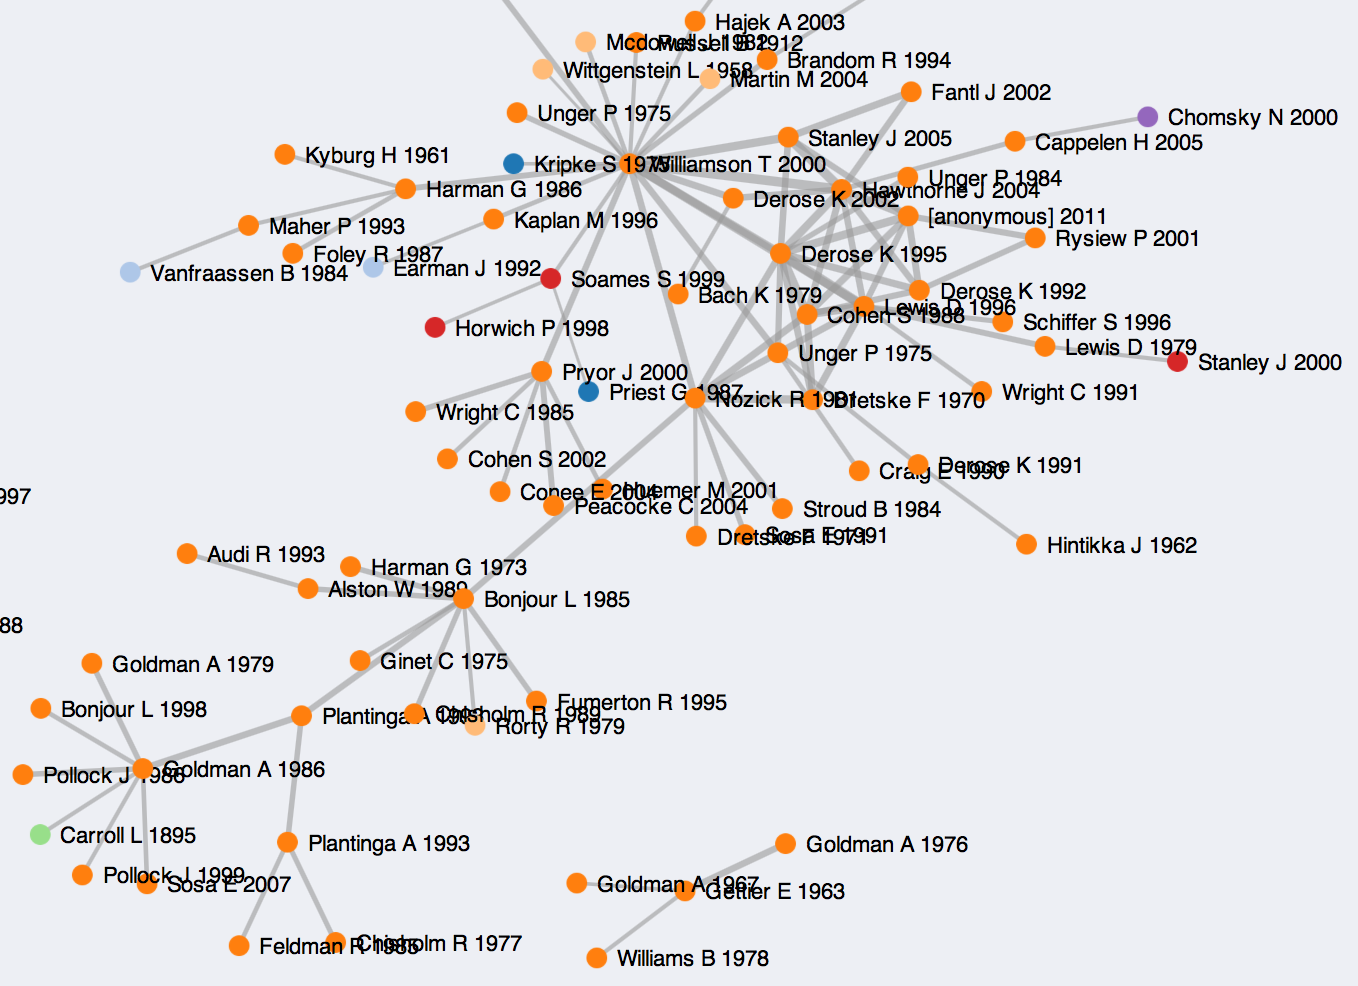
\includegraphics[width=1.0\textwidth]{img/citation_network}
      \label{fig:citation}
    \end{figure}
  \end{minipage}
  \begin{minipage}[t]{.4\textwidth}
    \begin{figure}[ht]
      \centering
      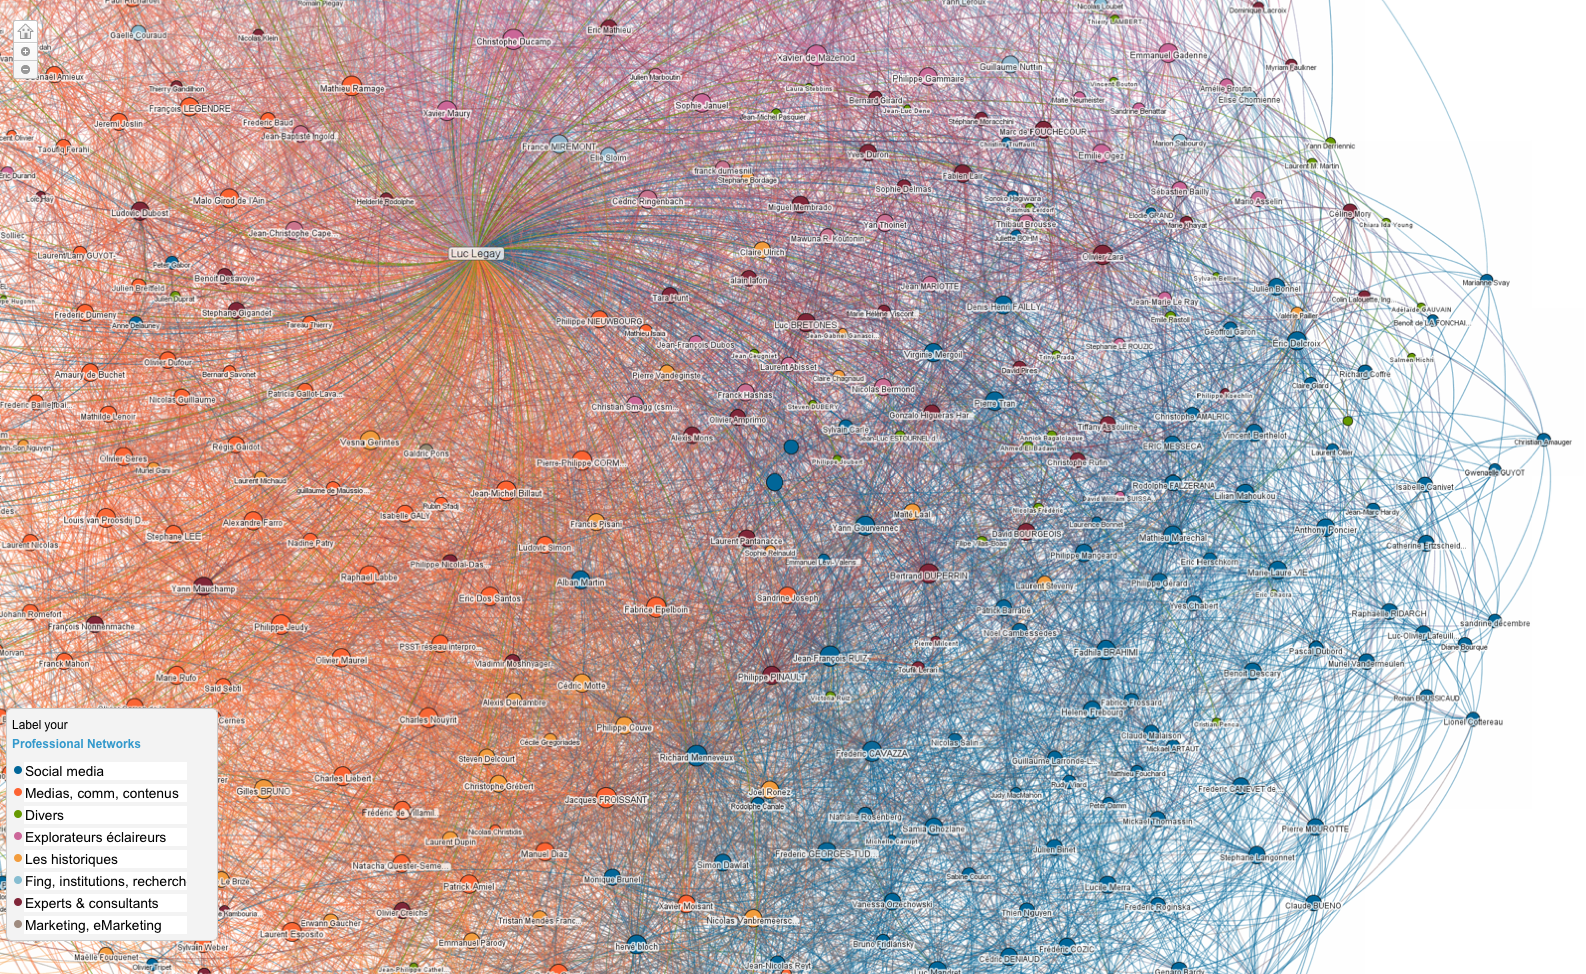
\includegraphics[width=1.0\textwidth]{img/linkedin}
      \label{fig:linkedin}
    \end{figure}
  \end{minipage}
\end{frame}
\begin{frame}{Why Do We Need Graph Convolutional Networks (cont'd)}
  \begin{minipage}[t]{.5\textwidth}
    Graphs vs Euclidean grids
    \begin{itemize}
    \item Irregular sampling
    \item Weighted edges
    \item No orientation (in general)
    \end{itemize}
    \vspace{1cm}
    Challenges
    \begin{enumerate}
    \item Formulate convolution on graphs
    \item Make them efficient
    \end{enumerate}
  \end{minipage}
  \begin{minipage}[t]{.4\textwidth}
    \begin{figure}[ht]
      \centering
      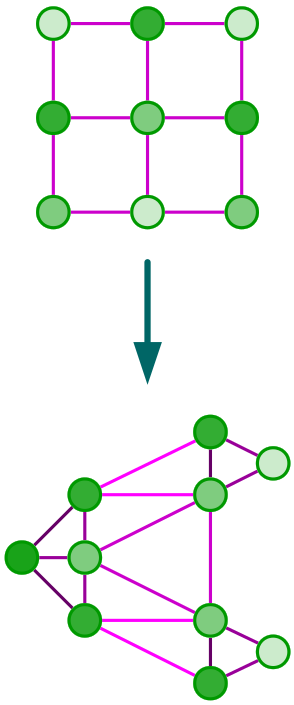
\includegraphics[width=1.0\textwidth, height=0.7\textheight, keepaspectratio]{img/problem}
      \label{fig:problem}
    \end{figure}

  \end{minipage}

\end{frame}
\begin{frame}{Outline}
    \tableofcontents
\end{frame}
\begin{frame}{Graph Gradient}
  \begin{minipage}[t]{\dimexpr.4\textwidth+2em}
    \begin{figure}[ht]
      \centering
      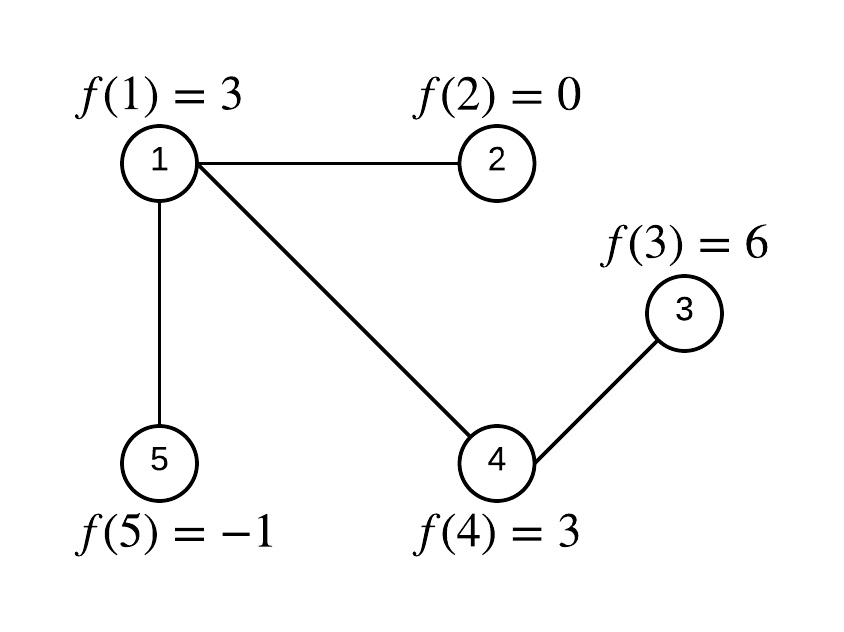
\includegraphics[width=1.0\textwidth, height=1.0\textheight, keepaspectratio]{img/graph_gradient}
      \label{fig:graph-gradient}
    \end{figure}
  \end{minipage}
  \begin{minipage}[t]{.5\textwidth}
    \begin{align*}
      f &:\mathcal{V} \rightarrow \mathbb{R} \\
      \nabla f &= { (f(v)-f(w)) }_{ v,w\in E } \\
    \end{align*}
    \begin{align*}
      E &= \left\{(1,2), (1,4), (1,5), \boldsymbol{(3,4)}\right\} \\
      \nabla f &= (-3,0,-4,\boldsymbol{3})
    \end{align*}
  \end{minipage}
  Limitations:
  \begin{enumerate}
  \item Directions arbitrarily
    \begin{itemize}
    \item Numerical properties of the gradient wouldn't be
        well-defined
    \end{itemize}
  \item Fix your reference point as a single vertex
    \begin{itemize}
    \item Gradient on edges going ``out of'' that vertex
    \end{itemize}
  \end{enumerate}
\end{frame}

\begin{frame}{Graph Gradient (cont'd)}
  Euclidean norm of the gradient:
  \[
  \sum _{ (v,w)\in E }^{  }{ { (f(v)-f(w)) }^{ 2 } } = { x }^{ T }\boldsymbol{A}x
  \]
  \begin{block}{Expressing a Quadratic Form with a Matrix}
    \begin{align*}
      ax^2 + 2bxy + cy^2 &= \begin{bmatrix} x & y \end{bmatrix}\begin{bmatrix} a & b \\ b & c \end{bmatrix}\begin{bmatrix} x \\ y \end{bmatrix} \\
      &= \begin{bmatrix} x & y \end{bmatrix} \begin{bmatrix} ax+by \\ bx+cy \end{bmatrix} \\
      &= x\left(ax+by\right) + y\left(bx+cy\right) \\
      &= ax^2 + 2bxy + cy^2
    \end{align*}
  \end{block}
\end{frame}

\begin{frame}{Graph Laplacian}
  \[
  L_{i,j} = \begin{cases}\text{deg}(v_i) & i = j\\ -A_{ij} & v_i  \sim v_j \\ 0 &\text{otherwise} \end{cases}
  \]
  \begin{align*}
    L &= D - A \in \mathbb{R}^{n \times n}: combinatorial \\
    \mathcal{L} &= D^{-\frac{1}{2}}LD^{-\frac{1}{2}}: normalized \\
    &= I_n - D^{-\frac{1}{2}}AD^{-\frac{1}{2}}
  \end{align*}
  \scalebox{0.6}{
    \begin{minipage}{\dimexpr.3\textwidth+2em}
      \begin{figure}[ht]
        \centering
        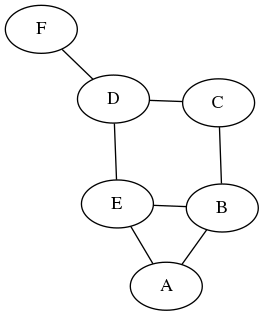
\includegraphics[width=1.0\textwidth,height=1.0\textheight, keepaspectratio]{img/laplacian}
        \label{fig:laplacian}
      \end{figure}
    \end{minipage}
  }
  \scalebox{0.55}{
    \begin{minipage}{\dimexpr.3\textwidth+2em}
      \[
      \kbordermatrix{
        & A & B & C & D & E & F \\
        A & 2 & 0 & 0 & 0 & 0 & 0 \\
        B & 0 & 3 & 0 & 0 & 0 & 0 \\
        C & 0 & 0 & 2 & 0 & 0 & 0 \\
        D & 0 & 0 & 0 & 3 & 0 & 0 \\
        E & 0 & 0 & 0 & 0 & 3 & 0 \\
        F & 0 & 0 & 0 & 0 & 0 & 1
      }
      \]
      \centering
      Degree Matrix
    \end{minipage}
  }
  \scalebox{0.55}{
    \begin{minipage}{\dimexpr.3\textwidth+2em}
      \[
      \kbordermatrix{
        & A & B & C & D & E & F \\
        A & 0 & 1 & 0 & 0 & 1 & 0 \\
        B & 1 & 0 & 1 & 0 & 1 & 0 \\
        C & 0 & 1 & 0 & 1 & 0 & 0 \\
        D & 0 & 0 & 1 & 0 & 1 & 1 \\
        E & 1 & 1 & 0 & 1 & 0 & 0 \\
        F & 0 & 0 & 0 & 1 & 0 & 0
      }
      \]
      \centering
      Adjacency Matrix
    \end{minipage}
  }
  \scalebox{0.55}{
    \begin{minipage}{\dimexpr.3\textwidth+2em}
      \[
      \kbordermatrix{
        & A & B & C & D & E & F \\
        A &  2 & -1 &  0 &  0 & -1 &  0 \\
        B & -1 &  3 & -1 &  0 & -1 &  0 \\
        C &  0 & -1 &  2 & -1 &  0 &  0 \\
        D &  0 &  0 & -1 &  3 & -1 & -1 \\
        E & -1 & -1 &  0 & -1 &  3 &  0 \\
        F &  0 &  0 &  0 & -1 &  0 &  1
      }
      \]
      \centering
      \hspace{1.55cm}Laplacian Matrix
    \end{minipage}
  }
\end{frame}
\begin{frame}{Linear Algebra}
  \begin{block}{Definition}
    A matrix $A$ is orthogonally diagonalizable if and only if there
    is an orthogonal matrix $U$ such that $A = UDU^{-1}$ where $D$ is
    a diagonal matrix.
  \end{block}
  \begin{block}{Remark}
    Recall that any orthogonal matrix $U$ is invertible and also that
    $U^{-1}=U^T$. Thus we can say that a matrix $A$ is orthogonally
    diagonalizable if there is a square matrix $U$ such that $A=UDU^T$
    where $D$ is a diagonal matrix.
  \end{block}
  \begin{block}{Remark}
    Any orthogonally diagonalizable $A$ must be symmetric.
    \[
    A^T=(UDU^T)^T=((U^T)^TD^TU^T=UDU^T=A
    \]
  \end{block}
\end{frame}
\begin{frame}{Graph Fourier Transform}
  L is symmetric and positive semidefinite (PSD) $\rightarrow L=U
  \Lambda U^T$ \textit{(EVD)}
  \begin{itemize}
  \item Graph Fourier basis $U=\left[u_0, \dots, u_{n-1}\right] \in \mathbb{R}^{n \times n}$
  \item Graph frequencies $\Lambda =\begin{bmatrix} \lambda _{ 1 } &  & 0 \\  & \ddots  &  \\ 0 &  & \lambda _{ n } \end{bmatrix} \in \mathbb{R}^{n \times n}$
  \end{itemize}
  \vspace{1cm}
  Graph Fourier Transform (GFT):
  \begin{itemize}
  \item Graph signal $f: \mathcal{V} \rightarrow \mathbb{R}$ seen as $\mathbb{R}^n$
  \item Transform: $\hat{f} = \mathcal{F}_{\mathcal{G}}\left\{ f \right\} = U^Tf \in \mathbb{R}^n$
  \item Inverse: $f = U\hat{f} = UU^Tf = f$
  \end{itemize}
\end{frame}
\begin{frame}{Graph Convolution}
  \footnotesize{
    \begin{block}{Convolution}
      \[u[t]\ast v[t]=\sum _{ k=-\infty  }^{ \infty  }{ u[k] v[t-k] }\]
      \[u[t]\ast v[t] \Leftrightarrow U[f]V[f]\]
    \end{block}
    \vspace{-0.6cm}
  \begin{align*}
    x\ast _{ \mathcal{G} }g &= \underbrace{U\underbrace { (U^Tg \odot U^Tx) }_{\mathcal{O}(n^2)}}_{\mathcal{O}(n^3)}  \\
    &=U(\hat{g} \odot U^Tx)
  \end{align*}
  Conveniently written as:
  \begin{align*}
    x \ast_{\mathcal{G}} g &= U\begin{bmatrix} \hat{g}(\lambda _{ 1 }) &  & 0 \\  & \ddots  &  \\ 0 &  & \hat{g}({\lambda _{ n }}) \end{bmatrix} U^Tx\\
    &= U \hat{g}(\Lambda)U^Tx \\
    &= \hat{g}(L)x
  \end{align*}
  }
\end{frame}
\begin{frame}{Graph Convolution (cont'd)}
  \[
  y = \hat{g}_{\theta}(L)x = U\hat{g}_{\theta}(\Lambda)U^Tx
  \]
  Non-parametric filter:
  \[
  \hat{g}_{\theta}(\Lambda) = \text{diag}(\theta), \theta \in \mathbb{R}^n
  \]
  \begin{itemize}
  \item Non-localized in vertex domain
  \item Learning complexity is $\mathcal{O}(n)$
  \end{itemize}
\end{frame}
\begin{frame}{Localized Filters}
  \begin{figure}
    \[
    \hat{g}_{\theta}(\Lambda) = \sum _{ k=0 }^{ K}{\theta_k\Lambda^k  }, \theta \in \mathbb{R}^K
    \]
    \caption*{\cite{hammond2011wavelets}}
  \end{figure}
  \begin{itemize}
  \item Value at j of $g_\theta$ centered at i: $(\hat{g}_\theta(L)\delta_i)_j = (\hat{g}_\theta(L))_{i,j}=\sum_{k}^{}{\theta_k(L^k)_{i,j}}$
  \item $d_\mathcal{G}(i,j)>K$ implies $(L^K)_{i,j}=0$
  \item K-localized
  \item Learning complexity is $\mathcal{O}(K)$
  \end{itemize}
\end{frame}
\begin{frame}{Recursive Formulation for Fast Filtering}
  \[
  \hat{g}_\theta(\Lambda) = \sum_{k=0}^{K}{\theta_kT_k(\hat\Lambda)}, \quad \tilde{\Lambda}=\frac{2}{\lambda_{max}}\Lambda - I_N
  \]
  \begin{itemize}
  \item Chebyshev polynomials: $T_k(x) = 2xT_{k-1}(x)-T_{k-2}(x)$ with $T_0(x)=1$ and $T_1(x)=x$
  \item Filtering: $y=\hat{g_\theta}(L)x=\sum_{k=0}^{K}{\theta_kT_k(\tilde{L})x}$
  \item Recurrence:
    $y=\hat{g}_\theta(L)x=[\bar{x}_0,\dots,\bar{x}_{K-1}]\theta$\\ where
    $\bar{x}_k=T_k(\tilde{L})x=2L\bar{x}_{k-1}-\bar{x}_{k-2}$ with
    $\bar{x}_0=x$ and $\bar{x_1}=\tilde{L}x$
    \item Computational complexity is $\mathcal{O}(K\mathcal{E})$
  \end{itemize}
\end{frame}
\begin{frame}{Recursive Formulation for Fast Filtering (cont'd)}
  When $K=1$:
  \begin{itemize}
  \item Alleviate the problem of overfitting on local neighborhood
    structures for graphs with very wide node degree distributions
  \item Allows us to build deeper models
    \begin{itemize}
    \item[--] Linear w.r.t. L and therefore a linear function on the
      graph Laplacian spectrum
    \end{itemize}
  \end{itemize}
  \begin{align*}
    y &= \hat{g}_\theta(L)x=\theta_0x+\theta_1(L-I_N)x=\theta_0x-\theta_1D^{-\frac{1}{2}}AD^{-\frac{1}{2}}x \\
    &= \theta\left(I_N+D^{-\frac{1}{2}}AD^{-\frac{1}{2}}\right)x
  \end{align*}
\end{frame}
\begin{frame}{Recursive Formulation for Fast Filtering (cont'd)}
  Constrain number of parameters to address overfitting by
  $\theta=\theta_0=-\theta_1$
  Renormalization trick: $I_N+D^{-\frac{1}{2}}AD^{-\frac{1}{2}} \rightarrow \tilde{D}^{-\frac{1}{2}}\tilde{A}\tilde{D}^{-\frac{1}{2}}$
  \begin{itemize}
  \item $I_N+D^{-\frac{1}{2}}AD^{-\frac{1}{2}}$ has eigenvalues in $[0,2]$
  \item Repeated application of this operation causes vanishing gradients
  \item $\tilde{A}=A+I_N$ and $\tilde{D}_{ii}=\sum_{j}^{}{\tilde{A}_{ij}}$
  \end{itemize}
  \begin{block}{General Formula}
    \[
    Z=\tilde{D}^{-\frac{1}{2}}\tilde{A}\tilde{D}^{-\frac{1}{2}}X\Theta
    \]
    where $X \in \mathbb{R}^{N \times C}$ and $\Theta \in \mathbb{R}^{C \times F}$
  \end{block}
\end{frame}
\begin{frame}{Example}
  \[
  Z=f(X,A)=\text{softmax}\left(\hat{A}\text{ReLU}\left(\hat{A}XW^{(0)}\right)W^{(1)}\right)
  \]
  \begin{itemize}
  \item $W^{(0)} \in \mathbb{R}^{C \times H}:$ input-to-hidden with H feature maps
  \item $W^{(1)} \in \mathbb{R}^{H \times F}:$ hidden-to-output
  \end{itemize}
  Cross-entropy error over all labeled examples:
  \[
  \mathcal{L} =-\sum_{l \in \mathcal{Y}_L}^{}{\sum_{f=1}^{F}{Y_{lf}\ln{Z_{lf}}}}
  \]
  where $\mathcal{Y}_L$ is the set of node indices that have labels
\end{frame}
\begin{frame}{Example (cont'd)}
  $W^{(0)}$ and $W^{(1)}$ are trained using batch gradient descent using the full dataset
  \begin{itemize}
  \item Sparse representation of $A$ requires $\mathcal{O}(\mathcal{E})$ memory
  \item Dropout is used for stochasticity in the training process
  \end{itemize}
\end{frame}

\section{Semi-Supervised Classification with GCN}
\begin{frame}{Node Classification}
  \small{
    \begin{block}{Problem}
      Classifying nodes in a graph where labels are only available for a
      small subset of nodes
    \end{block}
    \begin{align*}
      \mathcal{L} &= \mathcal{L}_0+\lambda\mathcal{L}_{reg} \\
      \mathcal{L}_{reg} &= \sum _{ i,j }^{  }{ { A }_{ ij }{ \left\| f({ X }_{ i })-f({ X }_{ j }) \right\|  }^{ 2 } } ={ f(X) }^{ T }\Delta f(X)
  \end{align*}
    \begin{block}{Idea}
      \begin{itemize}
      \item Encode the graph structure directly using a neural network
        model $f(X, A)$
      \item Train on a supervised target $\mathcal{L}_0$ for all nodes with labels
      \item Graph will allow the model to distribute gradient
        information from the $\mathcal{L}_0$
        \begin{itemize}
        \item[--] Learn representations of nodes both with and without labels
        \end{itemize}
      \end{itemize}
    \end{block}
  }
\end{frame}
\begin{frame}{Fast Approximate Convolutions on Graphs}
  \begin{figure}[H]
    \centering
    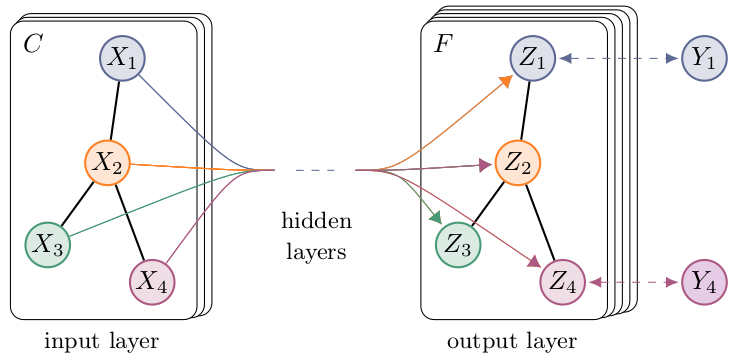
\includegraphics[width=1.0\textwidth, height=0.4\textheight, keepaspectratio]{img/gcn}
    \label{fig:gcn}
  \end{figure}
  \[
  { H }^{ (l+1) }=\sigma ({ \tilde { D }  }^{ -\frac { 1 }{ 2 }  }\tilde { A } { \tilde { D }  }^{ -\frac { 1 }{ 2 }  }{ H }^{ (l) }{ W }^{ (l) })
  \]
  \begin{itemize}
  \item $\tilde { A } =A+{ I }_{ N }$
  \item ${ \tilde { D }  }_{ ii }=\sum _{ j }^{  }{ { \tilde { A }  }_{ ij } } $
  \item $W^{(l)}$ is a trainable weight matrix
  \item $\sigma \left( \cdot  \right) $ is an activation function
  \item $H^{(l)} \in \mathbb{R}^{N \times D}$; $H^{(0)} = X$
  \end{itemize}
\end{frame}

\section{Experiments}
\begin{frame}{Experiments}
  \begin{figure}[H]
    \centering
    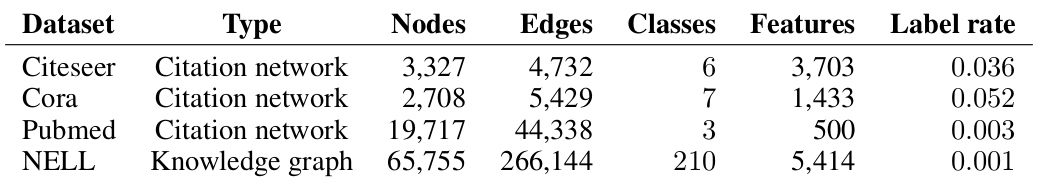
\includegraphics[width=1\textwidth, height=0.5\textheight, keepaspectratio]{img/dataset_stat}
    \label{fig:dataset}
  \end{figure}
  \vspace{-0.8cm}
  \begin{itemize}
  \item Citation networks:
    \begin{itemize}
    \item Documents are nodes,citation links are edges (undirected)
    \item Feature vectors: Sparse bag-of-words
    \item Sample 20 nodes uniformly at random for each class as training data, but all feature vectors
    \end{itemize}
  \item NELL:
    \begin{itemize}
    \item Nodes: 55864 (relation) + 9891 (entity) = 67755
    \item $(e_1,r,e_2) \rightarrow (e_1,r_1) \cup (e_2, r_2)$
    \item 61278-dim sparse feature vector per node (one-hot)
    \item Construct binary, symmetric adjacency matrix ($A_{ij}=1$ if one or more edges between nodes $i$ and $j$
    \end{itemize}
  \end{itemize}
\end{frame}
\begin{frame}{Experiments (cont'd)}
  \begin{figure}[H]
    \centering
    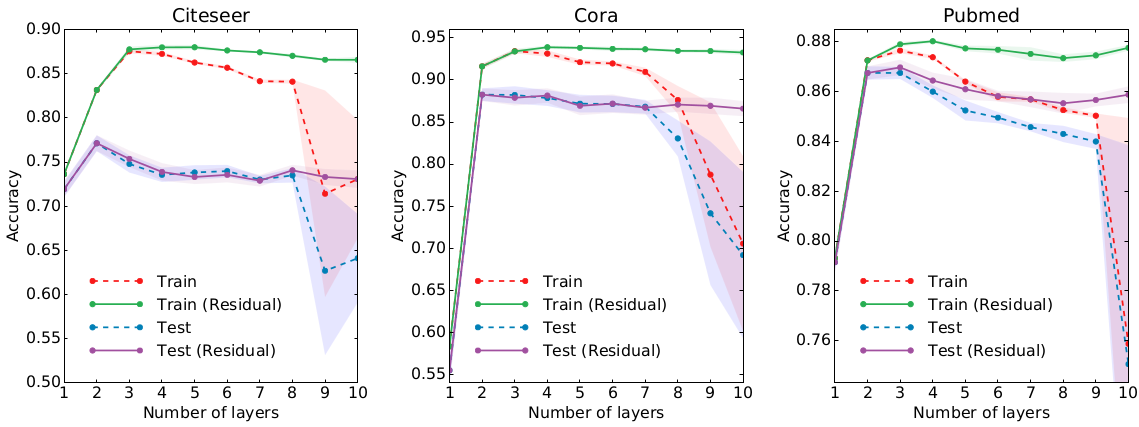
\includegraphics[width=1\textwidth, height=0.8\textheight, keepaspectratio]{img/model_depth}
    \label{fig:model_depth}
  \end{figure}
\end{frame}
\begin{frame}{Results}
  \begin{figure}[H]
    \centering
    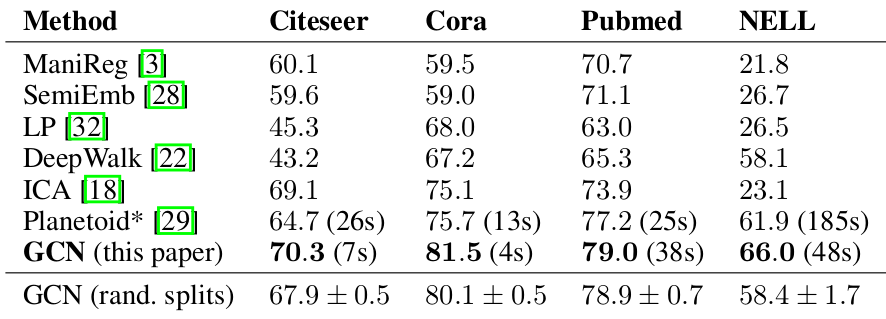
\includegraphics[width=1\textwidth, height=0.5\textheight, keepaspectratio]{img/comparison}
    \label{fig:comparison}
  \end{figure}
  \begin{itemize}
  \item Citeseer, Cora, and Pubmed: 0.5 (dropout rate), $5*10^{-4}$ (L2 regularization), 16 (number of hidden units)
    \item NELL: 0.1 (dropout rate), $1*10^{-5}$ (L2 regularization), 64 (number of hidden units)
  \end{itemize}
\end{frame}
\begin{frame}{Results (cont'd)}
  \begin{figure}[H]
    \centering
    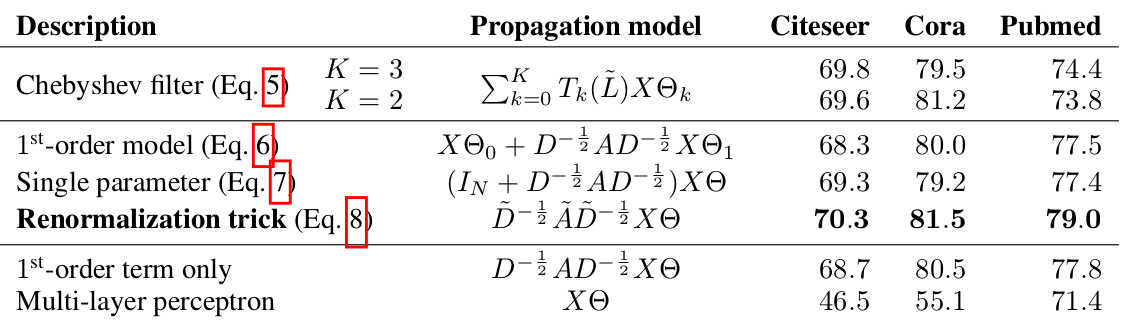
\includegraphics[width=1\textwidth, height=0.5\textheight, keepaspectratio]{img/propagation}
    \label{fig:propagation}
  \end{figure}
\end{frame}
\section{Conclusion}
\begin{frame}{Discussion}
  \begin{itemize}
  \item Graph-Laplacian regularization are limited due to their assumption
    that edges encode mere similarity of nodes
    \begin{itemize}
    \item[--] \cite{zhu2003semi}
    \item[--] \cite{belkin2006manifold}
    \item[--] \cite{weston2012deep}
    \end{itemize}
  \item Skip-gram based methods
    \begin{itemize}
    \item[--] multi-step pipeline which is difficult to optimize
    \item[--] \cite{mikolov2013distributed}, \cite{perozzi2014deepwalk}, \cite{tang2015line}, \cite{grover2016node2vec}
    \end{itemize}
    \item Proposed method supports propagation of feature information
      from neighboring nodes
      \begin{itemize}
      \item[--] improves classification accuracy
      \item[--] Only label information is aggregated in ICA
      \end{itemize}
  \end{itemize}
\end{frame}
\begin{frame}{Limitations and Future Work}
  \begin{itemize}
  \item Memory requirement: Full-batch gradient descent
    \begin{itemize}
    \item[--] Mini-batch stochastic gradient descent is a future work
    \end{itemize}
  \item Does not support edge features, and limited to undirected graphs
    \begin{itemize}
    \item[--] Solution: Represent the original directed graph as an undirected bipartite graph (NELL case)
    \end{itemize}
  \item Equal importance of self-connections vs. edges to neighboring nodes
    \[
    \tilde{A} = A + \lambda I_N
    \]
  \end{itemize}
\end{frame}
\begin{frame}{Questions}
  \begin{minipage}{\dimexpr.4\textwidth+4em}
    \centering
    \Huge{Questions?}
  \end{minipage}
  \begin{minipage}{.4\textwidth}
    \begin{figure}[ht]
      \centering
      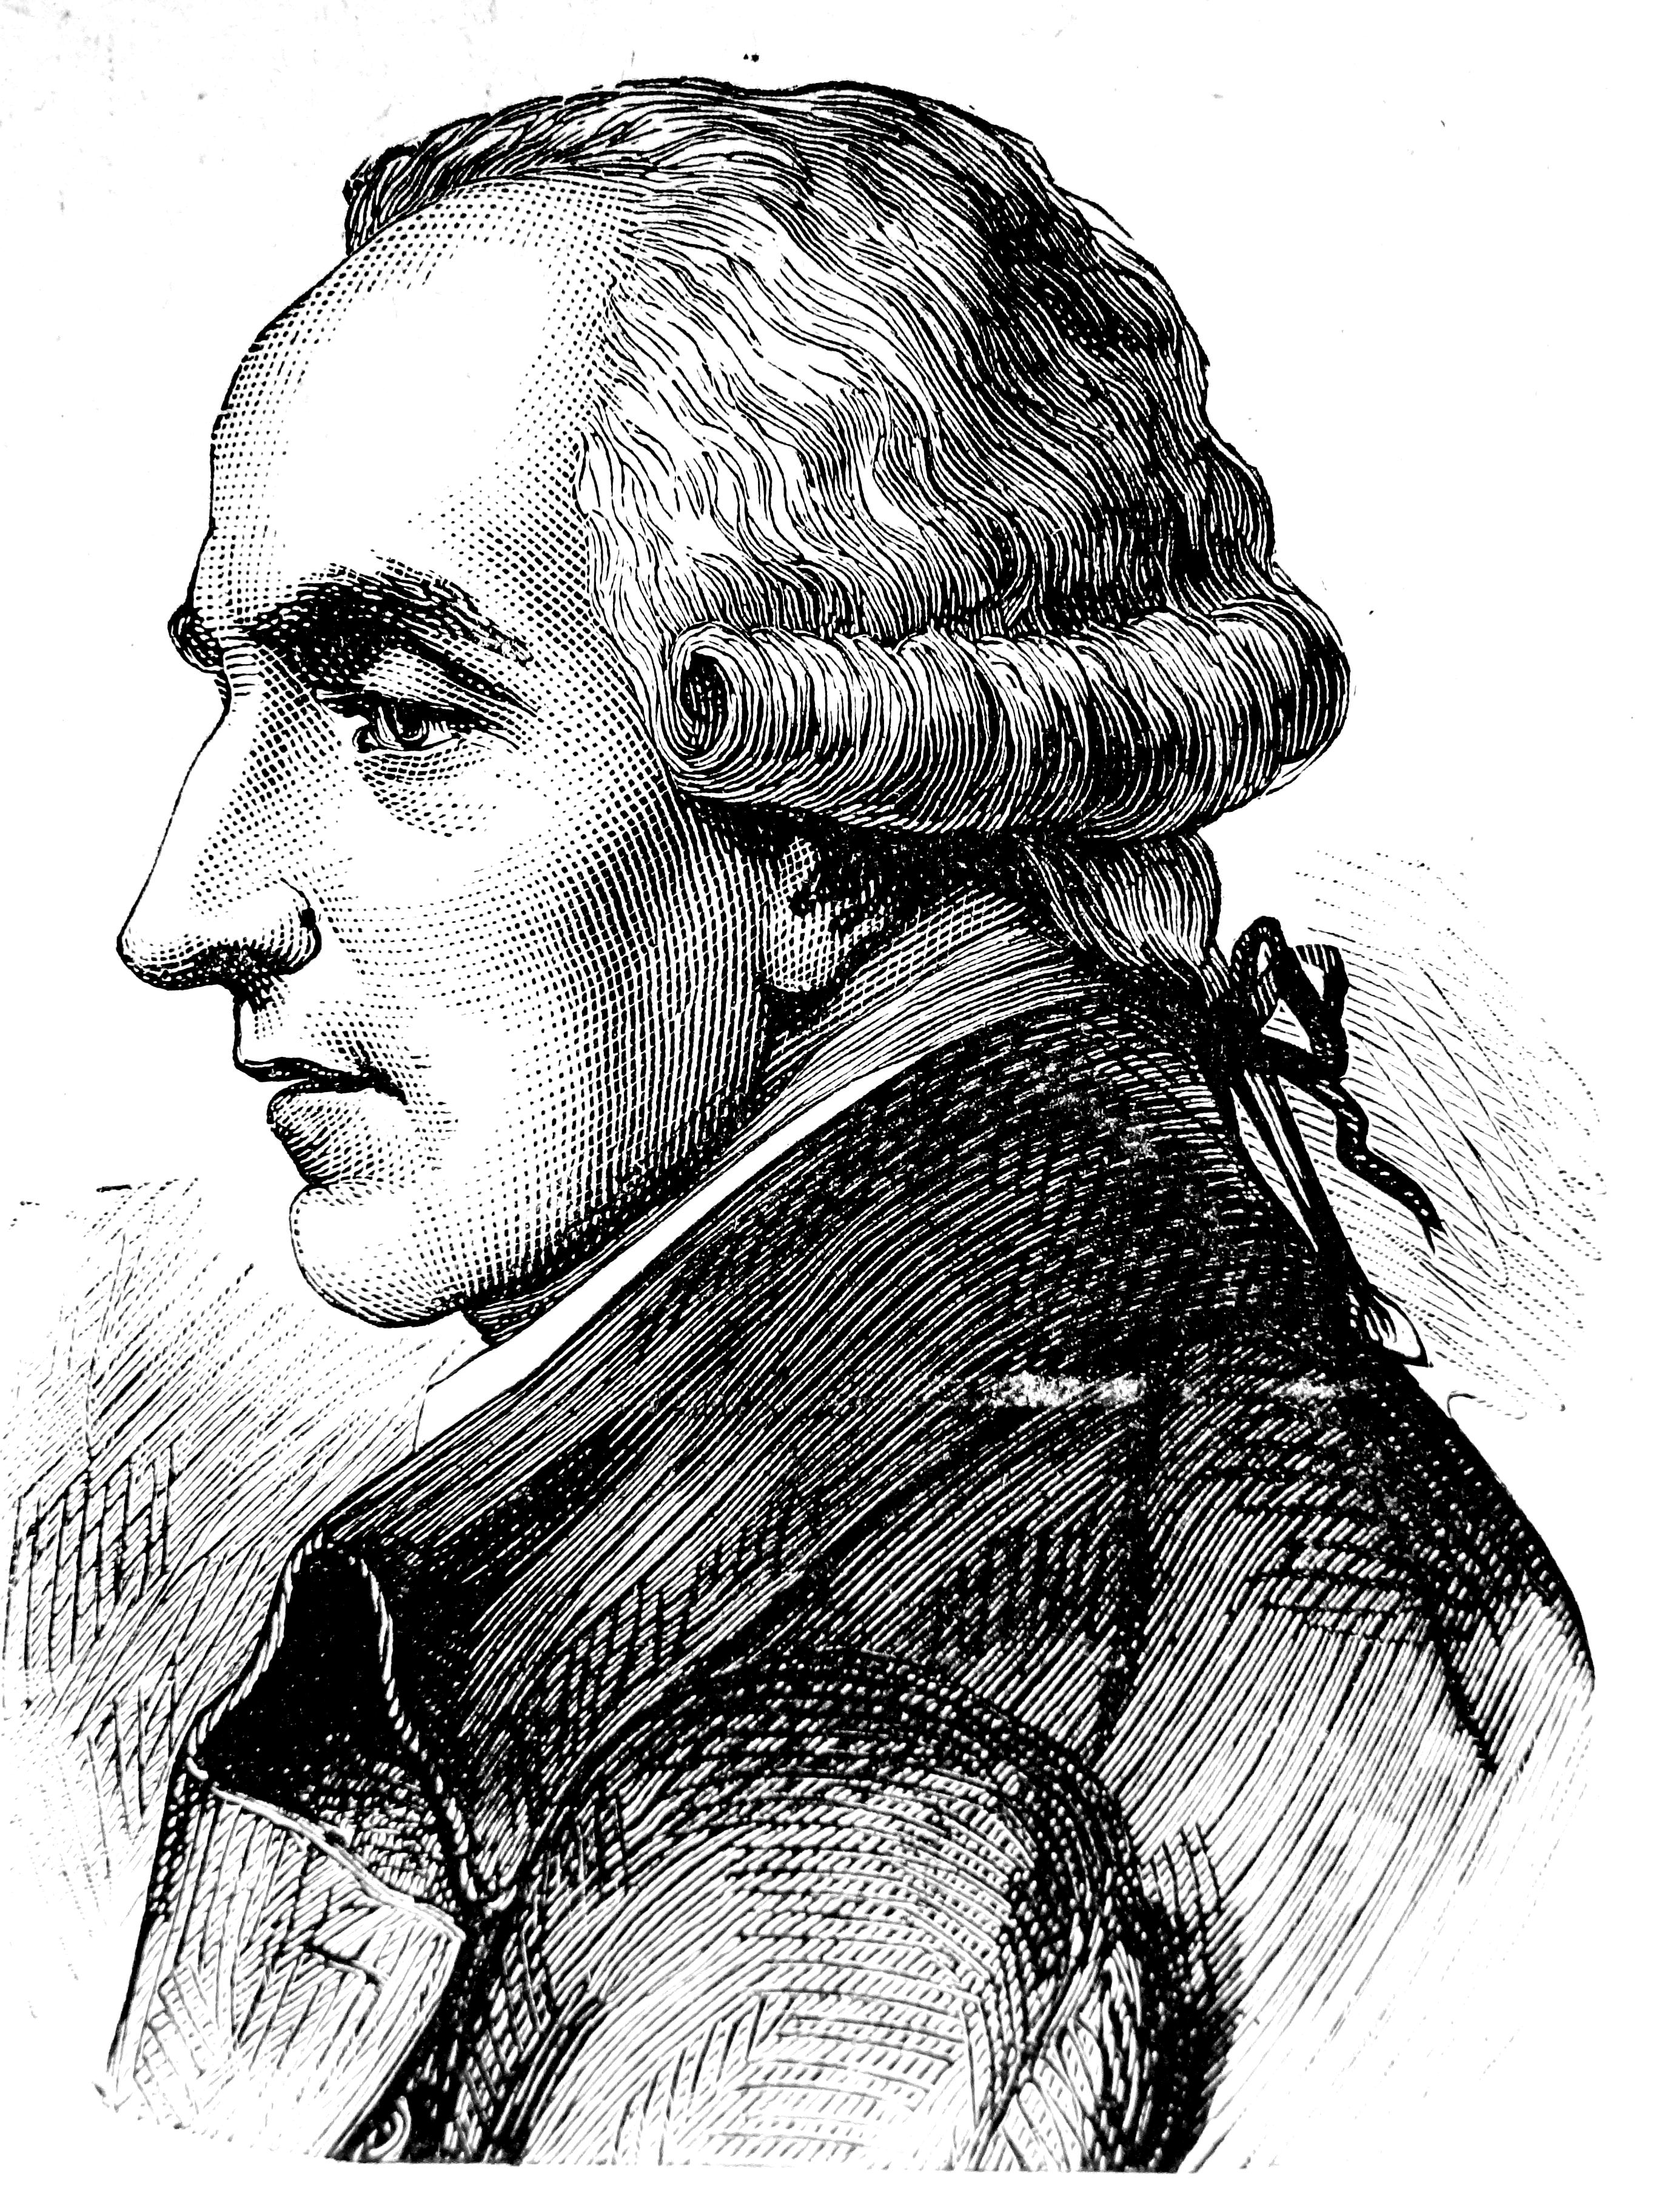
\includegraphics[width=1.0\textwidth, height=1.0\textheight, keepaspectratio]{img/laplace_profile}
    \end{figure}
  \end{minipage}
\end{frame}
\begin{frame}[allowframebreaks]
        \frametitle{References}
        \bibliographystyle{chicago}
        \bibliography{presentation}
\end{frame}
\end{document}
